\documentclass[a0,portrait]{a0poster}

\usepackage{multicol}
\columnsep=100pt
\columnseprule=3pt

\usepackage{times}
\usepackage{graphicx}
\graphicspath{{../}}
\usepackage{booktabs}
\usepackage[font=small,labelfont=bf]{caption}
\usepackage{amsfonts, amsmath, amsthm, amssymb, marvosym}
\usepackage{wrapfig}
\usepackage{enumitem}
\usepackage{fancyvrb}
\usepackage{xspace}
\usepackage[svgnames,usenames,dvipsnames]{xcolor}

%\usepackage{algorithm}
%\usepackage[noend]{algorithmic}
\usepackage{algpseudocode}

\def\texttts#1{\texttt{\large#1}}

\begin{document}

%---------------------------------------------------------------
%	POSTER HEADER 
%---------------------------------------------------------------
\begin{minipage}[b]{0.75\linewidth}
\veryHuge \color{NavyBlue} 
\textbf{Adversarial Hierarchical-Task Network para jogos em tempo real} 
\color{Black}\\[2cm] % Subtitle
\huge \textbf{Matheus de Souza Redecker e Felipe Rech Meneguzzi}\\
\Large Faculdade de Inform\'atica (FACIN) -- 
Pontif\'icia Universidade Cat\'olica do Rio Grande do Sul (PUCRS)\\ 
Porto Alegre -- RS -- Brasil\\ % University/organization
\Large \Letter ~ \texttt{matheus.redecker@acad.pucrs.br}\\
\Large \Letter ~ \texttt{felipe.meneguzzi@pucrs.br}\\
\\
\end{minipage}
\hspace*{-2cm}
\begin{minipage}[t]{0.25\linewidth}
\begin{center}
%era 12
\vspace{-15cm}
\includegraphics[width=9cm]{fig/logoPUCRS.pdf}%\\[-0.8cm]
\hspace*{1cm}
\end{center}
\end{minipage}

%---------------------------------------------------------------

\begin{multicols}{2} 
%---------------------------------------------------------------
%	ABSTRACT
%---------------------------------------------------------------
\color{NavyBlue}
\color{Black}
\raggedright
\Large

\newcommand\itemadjust{\itemsep.5em \parskip0pt \parsep0pt}
%---------------------------------------------------------------
%	Motivação
%---------------------------------------------------------------
\color{NavyBlue}
\section*{\huge Motiva\c{c}\~ao}
\color{Black}

\begin{itemize}
	[leftmargin=2em]\itemadjust
	\item Nos jogos de computador as rea\c{c}\~oes das jogadas devem ser quase que imediatas, por esse motivo t\'ecnicas que tentam explorar todas as possibilidades poss\'iveis de um jogo se tornam invi\'aveis para jogos com uma complexidade alta.
	\item Por exemplo, no xadrez a quantidade aproximada de estados poss\'iveis \'e de $10^{40}$, isso mostra que o poder de processamento para gerar, de maneira r\'apida, uma a\c{c}\~ao precisa ser alto. 
	\item O intuito deste trabalho é obter uma melhor performance na escolha das ações. Para isso, propomos a utilização do algoritmo de Adversarial Hierarchical-Task Network (AHTN)~\cite{ontanon2015adversarial}.
	\item Para rodar os experimentos escolhemos a plataforma MicroRTS~\cite{ontanon2013combinatorial}, que \'e um jogo de estrat\'egia em tempo real. 
\end{itemize}
%Qual o problema?;
%Pq é interessante?; e
%O que tu te propoe a fazer?
%---------------------------------------------------------------
%   Background
%---------------------------------------------------------------
\color{NavyBlue}
\section*{\huge Background}
\color{Black}

\textbf{Adversarial Hierarchical-Task Network}

\begin{itemize}
	[leftmargin=2em]\itemadjust
	\item O AHTN \'e um algoritmo desenvolvido para lidar com o problema do grande fator de ramifica\c{c}\~ao dos jogos em tempo real.
	\item Ele utiliza conhecimento de dom\'inio no estilo de planejamento hier\'arquico (HTN).
	\item No algoritmo s\~ao combinados t\'ecnicas de HTN com o algoritmo \textit{minimax search}.
	\item O algoritmo assume jogos totalmente observ\'aveis, baseados em turno e determin\'isticos. 
\end{itemize}

\vspace{10mm}

{\small
\begin{algorithmic}[1]
	\Function {AHTNMax}{$s, N_{+}, N_{-}, t_{+}, t_{-}, d$}
	\If {$terminal(s) \vee d \leq 0$}\label{alg:lin:firstLine}
	\State	\Return $(N_{+}, N_{-}, e(s))$
	\EndIf
	\If {$nextAction(N_{+}, t_{+}) \neq \perp$} \label{alg:ahtn:nexaction}
	\State $t = nextAction(N_{+}, t_{+})$ 
	\State \Return $\Call{AHTNMin}{(\gamma(s,t), N_{+}, N_{-}, t, t_{-}, d-1)}$ \label{alg:ahtn:troca}
	\EndIf
	\State $N_{+}^{*} = \perp, N_{-}^{*} = \perp, v^{*} = -\infty$
	\State $\aleph = decompositions_{+}(s, N_{+}, N_{-}, t_{+}, t_{-})$ \label{alg:decompositions}
	\ForAll{$N \in \aleph$} \label{alg:ahtn:for}
	\State $(N^{'}_{+}, N^{'}_{-}, v^{'}) = AHTNMax(s, N, N_{-}, t_{+}, t_{-}, d)$
	\If{$v^{'} > v^{*}$}
	\State $N_{+}^{*} = N^{'}_{+}, N_{-}^{*} = N^{'}_{-}, v^{*} = v^{'} $
	\EndIf
	\EndFor		
	\State \Return $(N_{+}^{*}, N_{-}^{*}, v^{*} )$
	\EndFunction
\end{algorithmic}
}

\vspace{15mm}
\textbf{Simple Hierarchical Ordered Planner 2}
\begin{itemize}
	[leftmargin=2em]\itemadjust
	\item Simple Hierarchical Ordered Planner 2 (SHOP2) \'e um sistema de planejamento independente de dom\'inio baseado em planejamento hier\'arquico (HTN)~\cite{nau2003shop2}.
	\item O SHOP2 precisa de uma descrição do dom\'inio e uma descrição do problema para gerar os planos.
	\item A descrição do dom\'inio é a descri\c{c}\~ao do dom\'inio de planejamento, onde estão descritos os m\'etodos e operadores.
	\item Já a descrição do problema, é onde está descrito o estado inicial as tarefas que desejam ser alcançadas.
\end{itemize}


\vspace{15mm}
\textbf{MicroRTS}


\begin{itemize}
	[leftmargin=2em]\itemadjust
	\item O MicroRTS \'e um jogo de estrat\'egia em tempo real (RTS).
	\item Ele \'e uma simplifica\c{c}\~ao do jogo Starcraft, feito por Santiago Onta\~n\'on.
	\item O MicroRTS foi desenvolvido para fins acad\^emicos, com o intuito de aplicar e desenvolver t\'ecnicas de Intelig\^encia Artificial.
\end{itemize}

\vspace{10mm}

\begin{center}
	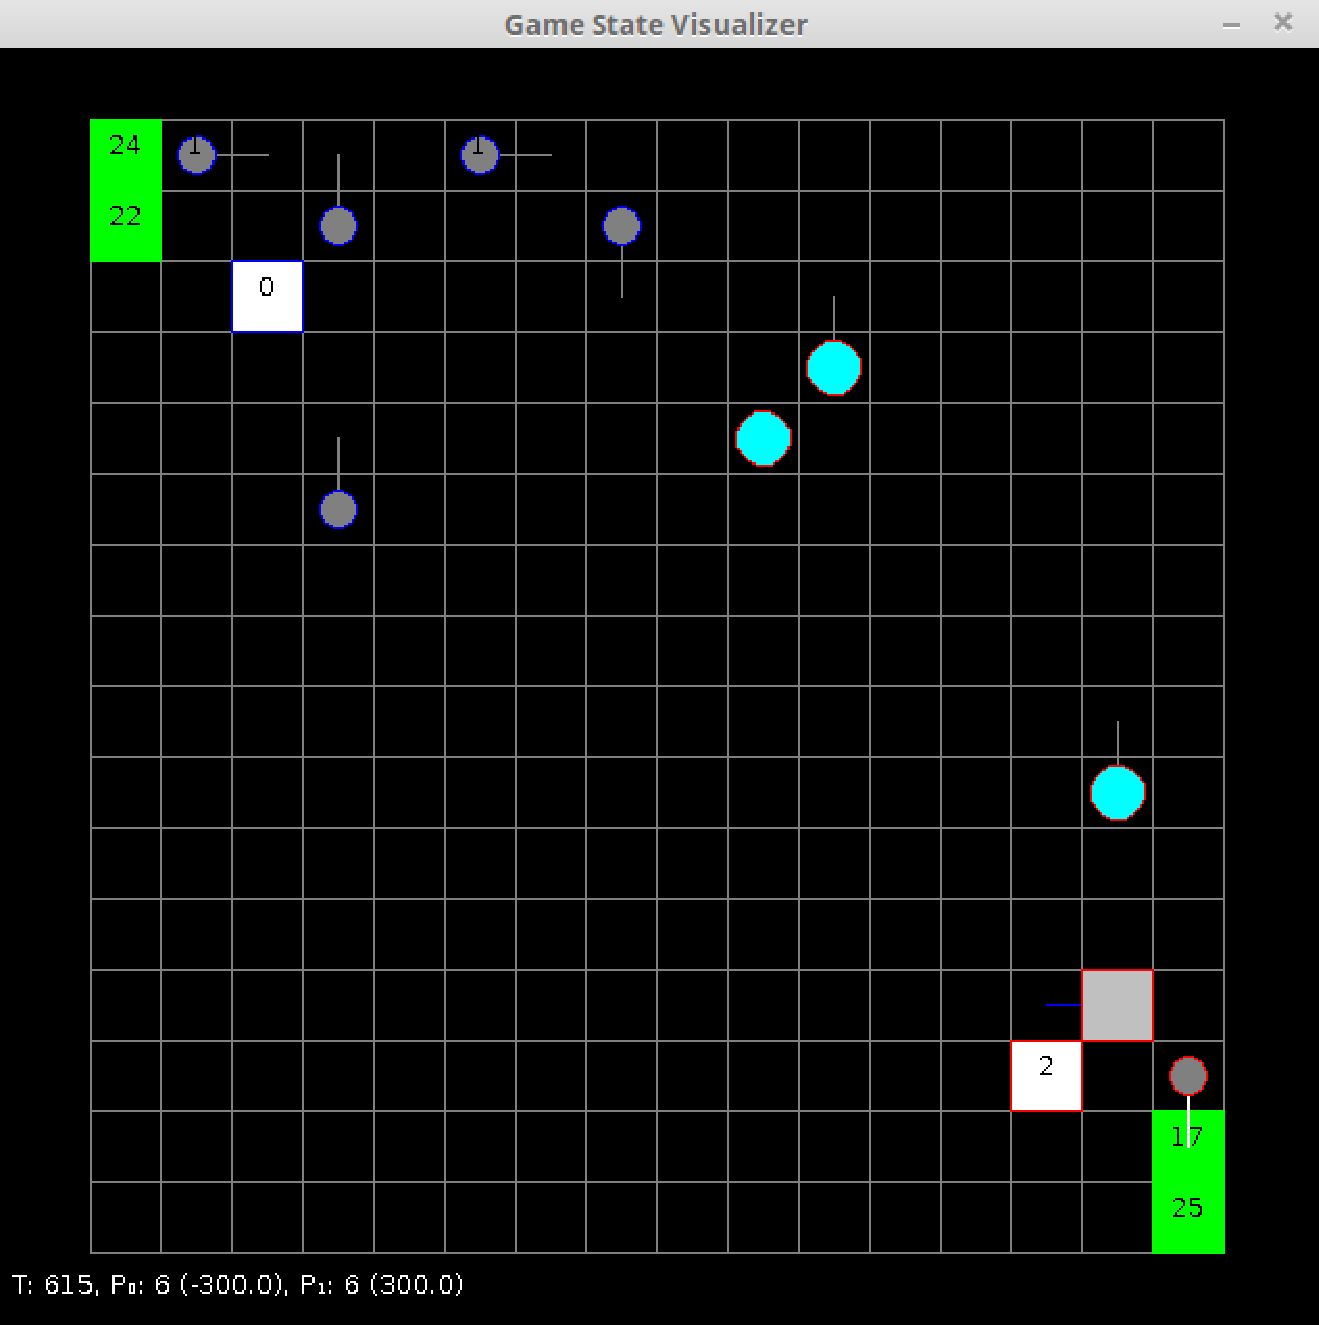
\includegraphics[width=0.5\linewidth]{fig/microRts.pdf}
	\captionof{figure}{Exemplo de tela de um jogo do MicroRTS.}
\end{center}	


%---------------------------------------------------------------
%	Implementação
%---------------------------------------------------------------
\color{NavyBlue}
\section*{\huge Implementa\c{c}\~ao}
\color{Black}

\begin{itemize}
	[leftmargin=2em]\itemadjust
	\item A implementa\c{c}\~ao do algoritmo foi feita na plataforma do MicroRTS, utilizando o SHOP2 para gera\c{c}\~ao dos planos.
	\item Foram criados dois conhecimento de dom\'inio pensando em um cen\'ario de jogo onde o jogador cria tropas para mandar atacar.
	\item A primeira estrat\'egia cria apenas uma unidade de ataque por vez e em seguida manda atacar. Já a segunda estrat\'egia enquanto está atacando também cria novas tropas.  
\end{itemize}


%---------------------------------------------------------------
%	Experimentos e Resultados
%---------------------------------------------------------------
\color{NavyBlue}
\section*{\huge Experimentos e resultados}
\color{Black}

\begin{itemize}
	[leftmargin=2em]\itemadjust
	\item Os experimentos a seguir foram executados em um mapa 16 por 16, com cada jogador inicialmente possuindo uma base, um trabalhador e dois recursos pr\'oximos a sua base. 
	\item O MicroRTS possui algumas t\'ecnicas de jogo implementadas, que podem ser jogados contra.
	\item O algoritmo de AHTN foi testado contra algumas dessas t\'ecnicas começando dos dois lados do jogo, azul na parte superior, e vermelho na parte inferior.
\end{itemize}

\vspace{10mm}

{\small
\begin{center}
	\begin{tabular}{|c|cc|cc|}
		\hline
		\textbf{}           & \multicolumn{2}{c|}{\textbf{Lado Azul}}                    & \multicolumn{2}{c|}{\textbf{Lado Vermelho}}                \\ \hline
		\textbf{Advers\'ario} & \multicolumn{1}{c|}{\textbf{Vitorias}} & \textbf{Derrotas} & \multicolumn{1}{c|}{\textbf{Vit\'orias}} & \textbf{Derrotas} \\ \hline
		\multicolumn{5}{|c|}{\textbf{Estrat\'egia 1}}                                                                                                   \\ \hline
		Random              & 5                                      & 0                 & 5                                      & 0                 \\
		Ranged              & 0                                      & 5                 & 5                                      & 0                 \\
		Heavy               & 0                                      & 5                 & 5                                      & 0                 \\
		Light               & 0                                      & 5                 & 5                                      & 0                 \\
		Worker              & 0                                      & 5                 & 0                                      & 5                 \\ \hline
		\multicolumn{5}{|c|}{\textbf{Estrategia 2}}                                                                                                   \\ \hline
		Random              & 5                                      & 0                 & 5                                      & 0                 \\
		Ranged              & 5                                      & 0                 & 5                                      & 0                 \\
		Heavy               & 0                                      & 5                 & 5                                      & 0                 \\
		Light               & 0                                      & 5                 & 5                                      & 0                 \\
		Worker              & 0                                      & 5                 & 0                                      & 5                 \\ \hline
	\end{tabular}
\captionof{table}{Resultado do algoritmo contra t\'ecnicas do MicroRTS.}
\end{center}
}

%\begin{center}
%	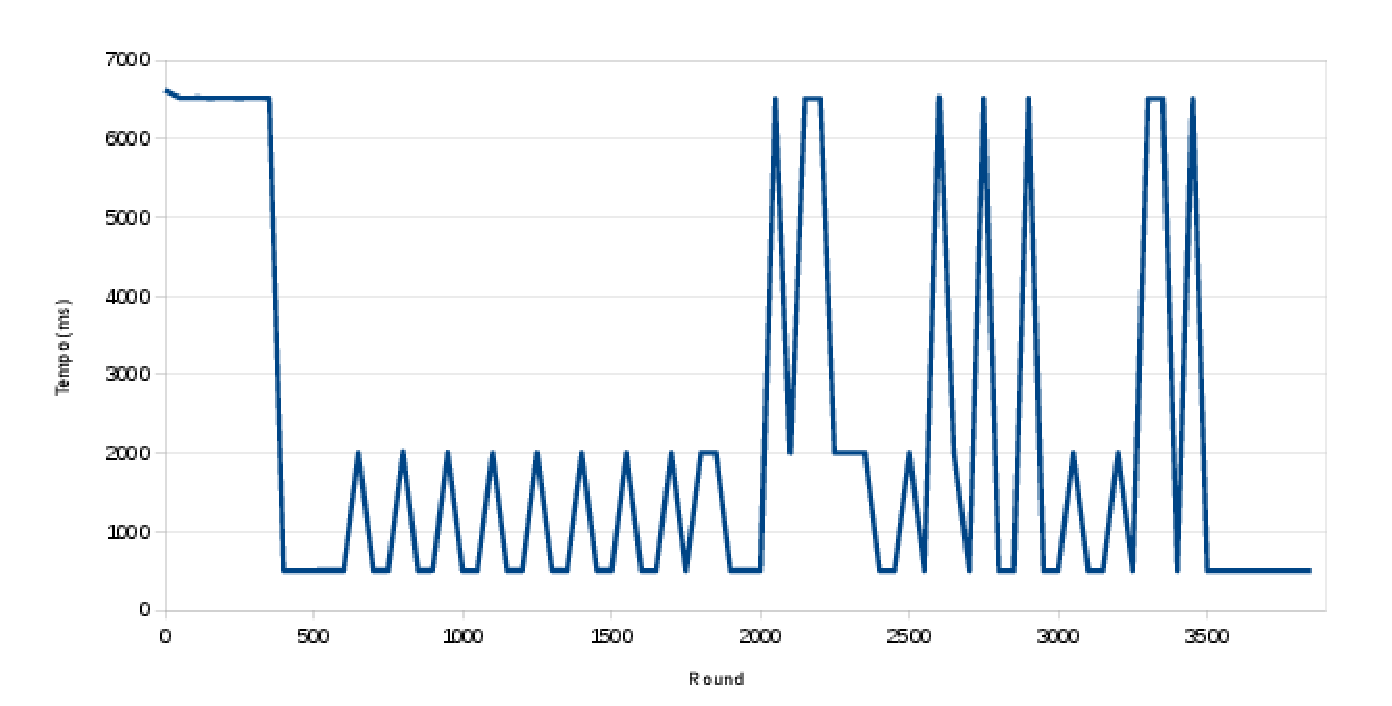
\includegraphics[width=0.8\linewidth]{fig/graph.pdf}
%	\captionof{figure}{Tempo levado pelo algoritmo em cada round.}
%\end{center}	


\vspace{13mm}



%---------------------------------------------------------------
% 	Conclusão
%---------------------------------------------------------------
%\vspace{-12mm}
%\color{NavyBlue}
%\section*{\huge Conclus\~ao}
%\color{Black}

%We have shown empirically that our approach yields not only superior accuracy results but also substantially faster recognition times for all used domains in evaluating against Ram{\'{\i}}rez and Geffner's approach~\cite{RamirezG_IJCAI2009}.

%\begin{itemize}[leftmargin=2em]\itemadjust
%	\item This work addresses the gap in existing norm identification approaches, which assume that violations do not occur, or that when they occur a violation signal is always generated
%	\item We consider two types of evidence:
%	\begin{itemize}
%		%\item Behaviour that is not necessarily always compliant
%                \item Observed traces of other agents, assumed to be generated by plans
%		\item Violation signals, which may be emitted following norm violation
%	\end{itemize}
%	\item An agent using our approach generates norm-compliant behaviour at least $70\%$ in the presence of a large number of norms
%\end{itemize}

%---------------------------------------------------------------
%	Referencias
%---------------------------------------------------------------
\vspace{-9mm}
\large
\color{NavyBlue}
\section*{Refer\^encias}
\renewcommand{\section}[2]{}
\color{Black}
\raggedright
\bibliographystyle{plain}
\bibliography{poster}

\end{multicols}
%---------------------------------------------------------------
%	Agradecimentos?
%---------------------------------------------------------------
%\vspace{-0.5cm}
%\hrulefill
%\normalsize
%\vspace{-1cm}
%\section*{Agradecimentos}
%\vspace{-1cm}
%This research was carried out in cooperation with HP Brazil using incentives of the Brazilian Informatics Law (\# 8.2.48 of 1991).

%----------------------------------------------------------------------------------------
\end{document}